\section{Results}

% Result text is placeholder until its seal's run completes. No result number appears here unless it is copied
% from a named file, and that file is cited in a comment beside it.
% Figure files are referenced by relative path (../../results/...). A missing file renders a pending stub.
\newcommand{\stub}[2]{\begin{minipage}[t]{0.48\linewidth}\centering\pendingbox{#2}\\[0.3em]\textbf{#1}\end{minipage}}

\subsection{Fig 1: reference model}

\begin{figure}[tbp]
\centering
\IfFileExists{../../results/viz/schema/t1_kd1p41_n4000_s1_T8_schema.png}{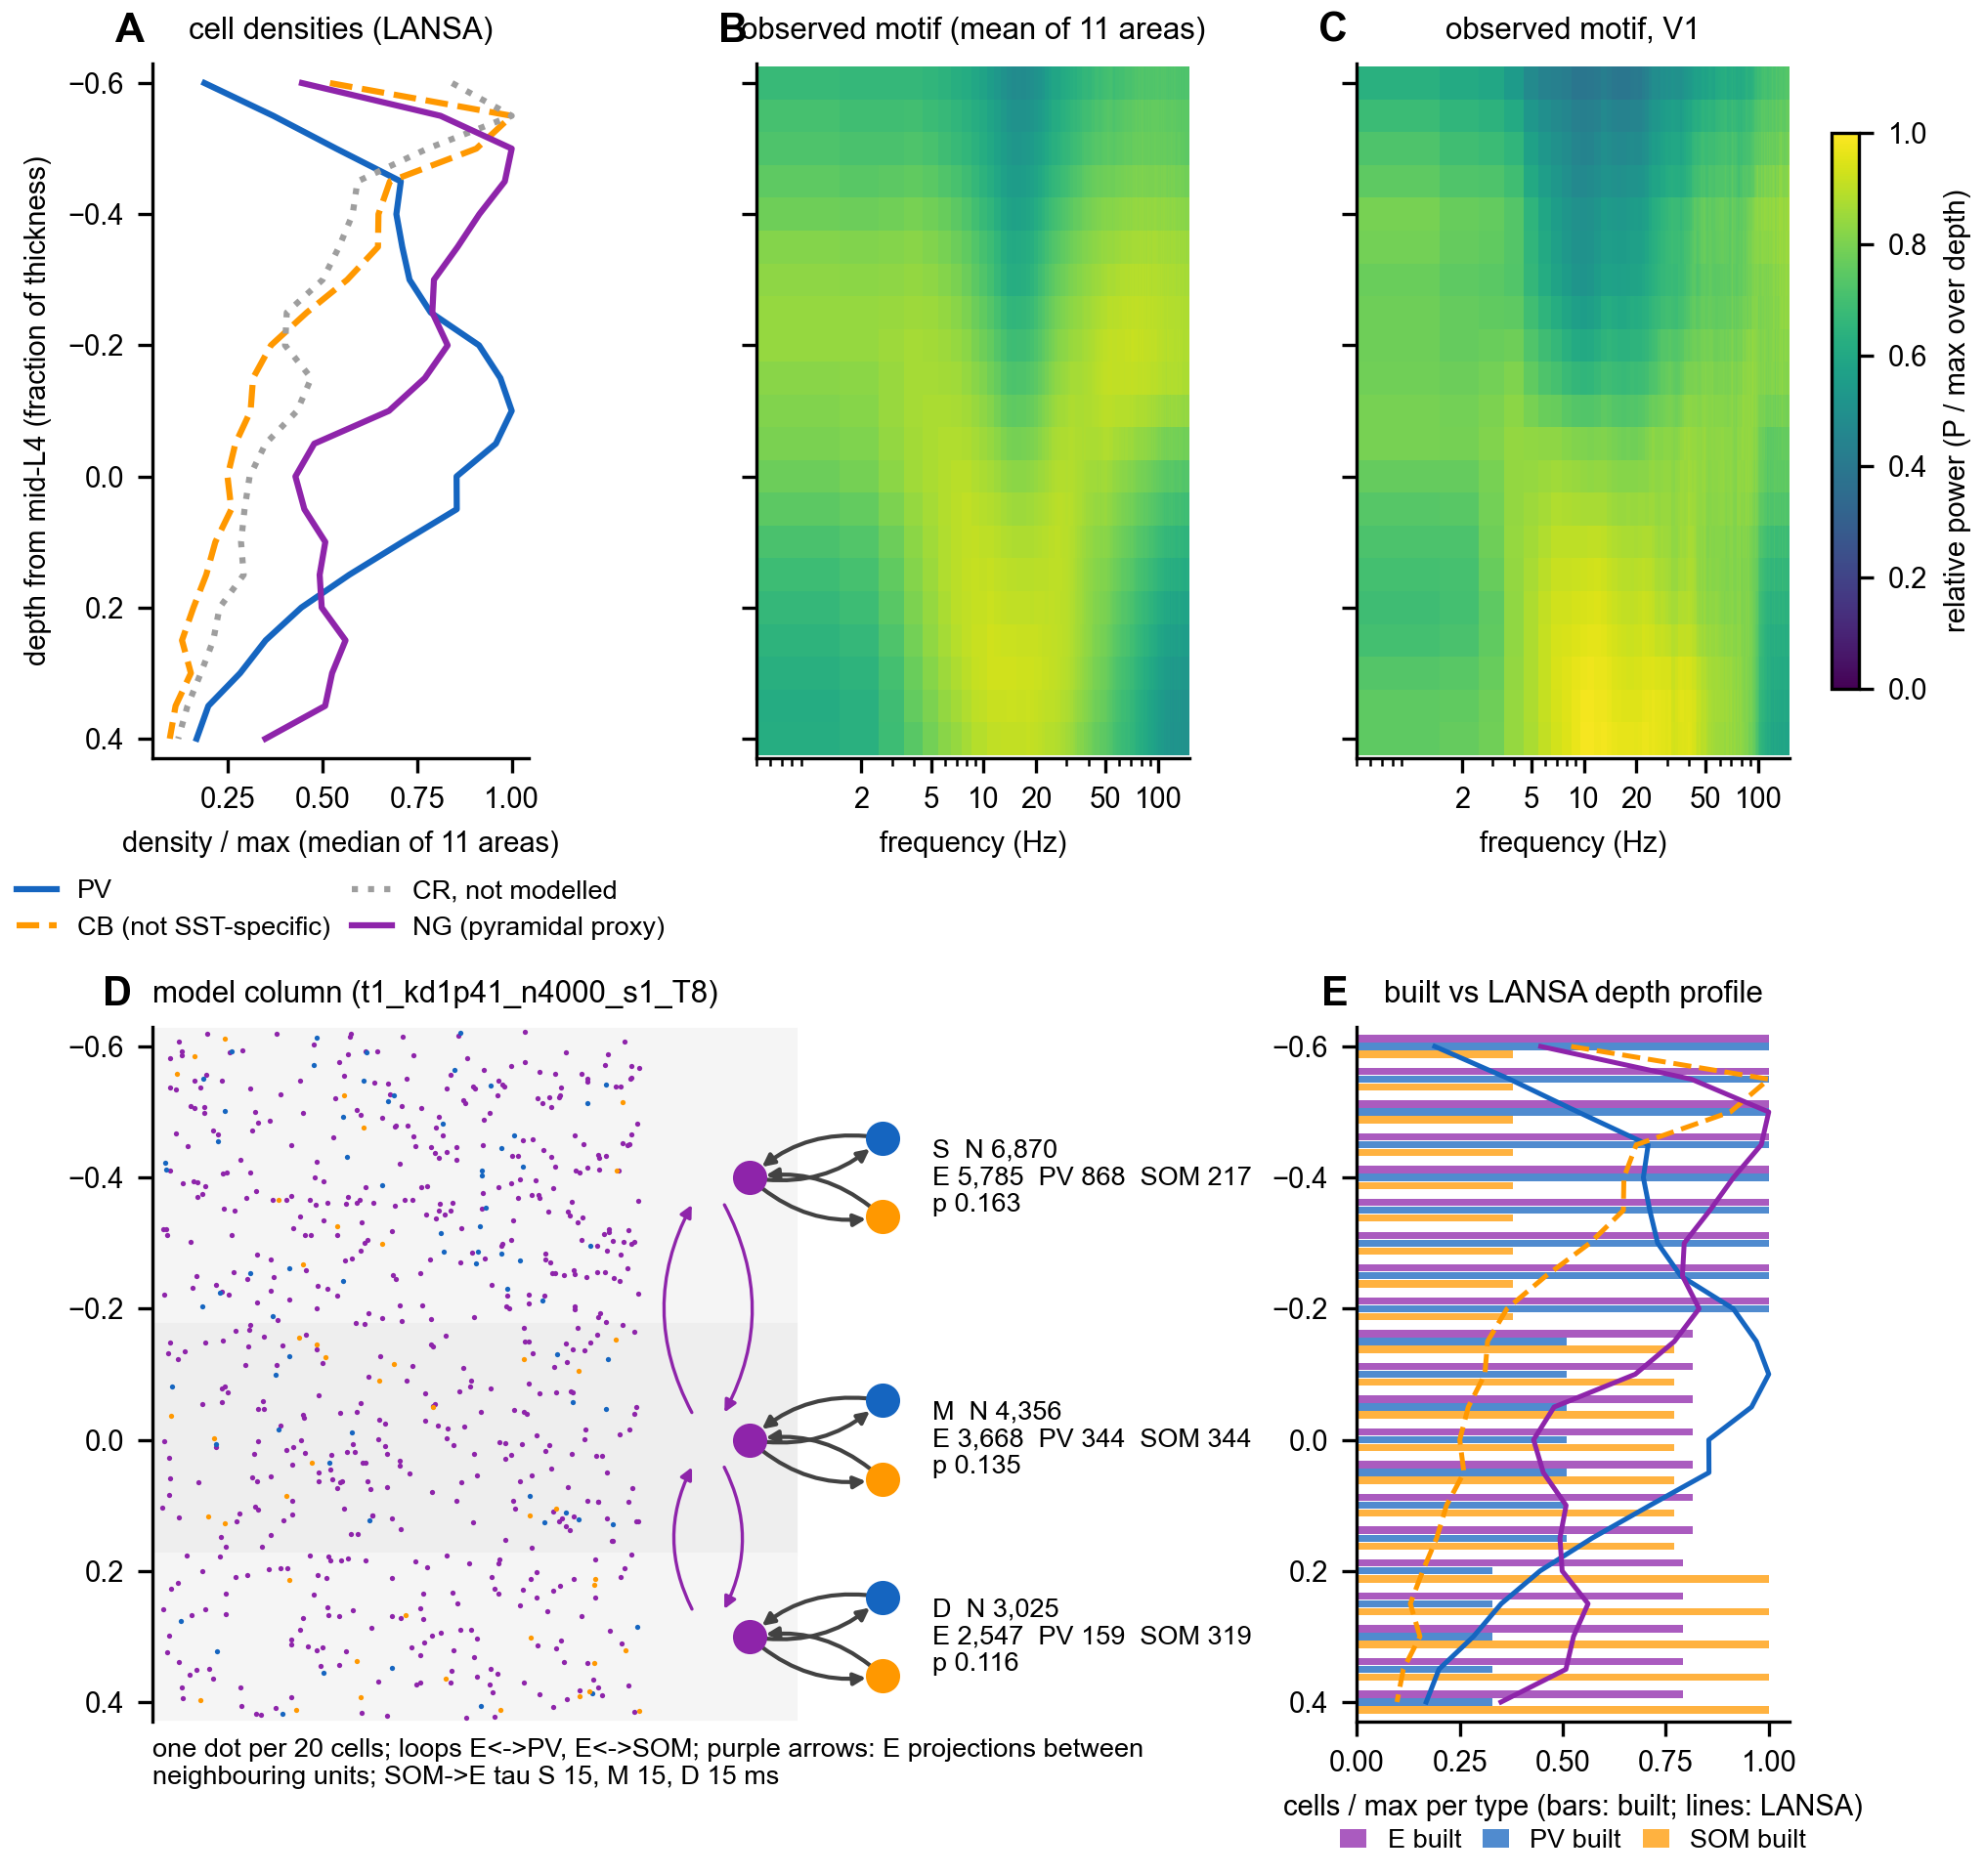
\includegraphics[width=\linewidth]{../../results/viz/schema/t1_kd1p41_n4000_s1_T8_schema.png}}{\pendingbox{data and circuit schema}}
\caption{Data and circuit (layout after Herrera 2026; \texttt{scripts/e2\_circuit\_schema.py}). A: LANSA cell densities
per type against depth from mid-L4, median of 11 areas, each type divided by its maximum (CB taken as SST, CR as VIP,
NG as the pyramidal proxy). B, C: observed relative power, mean of the 11 areas and V1. D: the T1 model
(\texttt{e2\_3unit\_n4000\_dens\_k1\_kd1p41\_sst15}) as built, one dot per 20 cells in each unit's depth bins, with its
within-unit loops and inter-unit E projections. E: built cells per type and depth bin against the LANSA profiles. LANSA
densities are relative per type, so E compares depth profiles only. No panel is simulated.}
\end{figure}

\todo{Fig 1 text: the reference model kd1\_sst15 at n4000, seed 1; its architecture, raster, spectra, SL maps, LFP and CSD; the observed LANSA map.}

\begin{figure}[tbp]
\centering
\panel{A}{../../results/viz/paper_w3/sw_n4000_dens_k1_kd1_sst15_s1_T8_V0_architecture.png}{0.85\linewidth}{V0 architecture}
\caption{Reference model \texttt{e2\_3unit\_n4000\_dens\_k1\_kd1\_sst15}, seed 1, 8 s run, 2 s discarded; an exploratory
E2 run (see the software status in Methods). A: architecture from the V0 file (paper\_w3). The details table (cell
numbers and types per unit, edges per rule, parameters with their sources) is Tables~S1--S4.}
\end{figure}

\begin{figure}[tbp]
\centering
\IfFileExists{../../results/viz/paper_w3/sw_n4000_dens_k1_kd1_sst15_s1_T8_block.png}{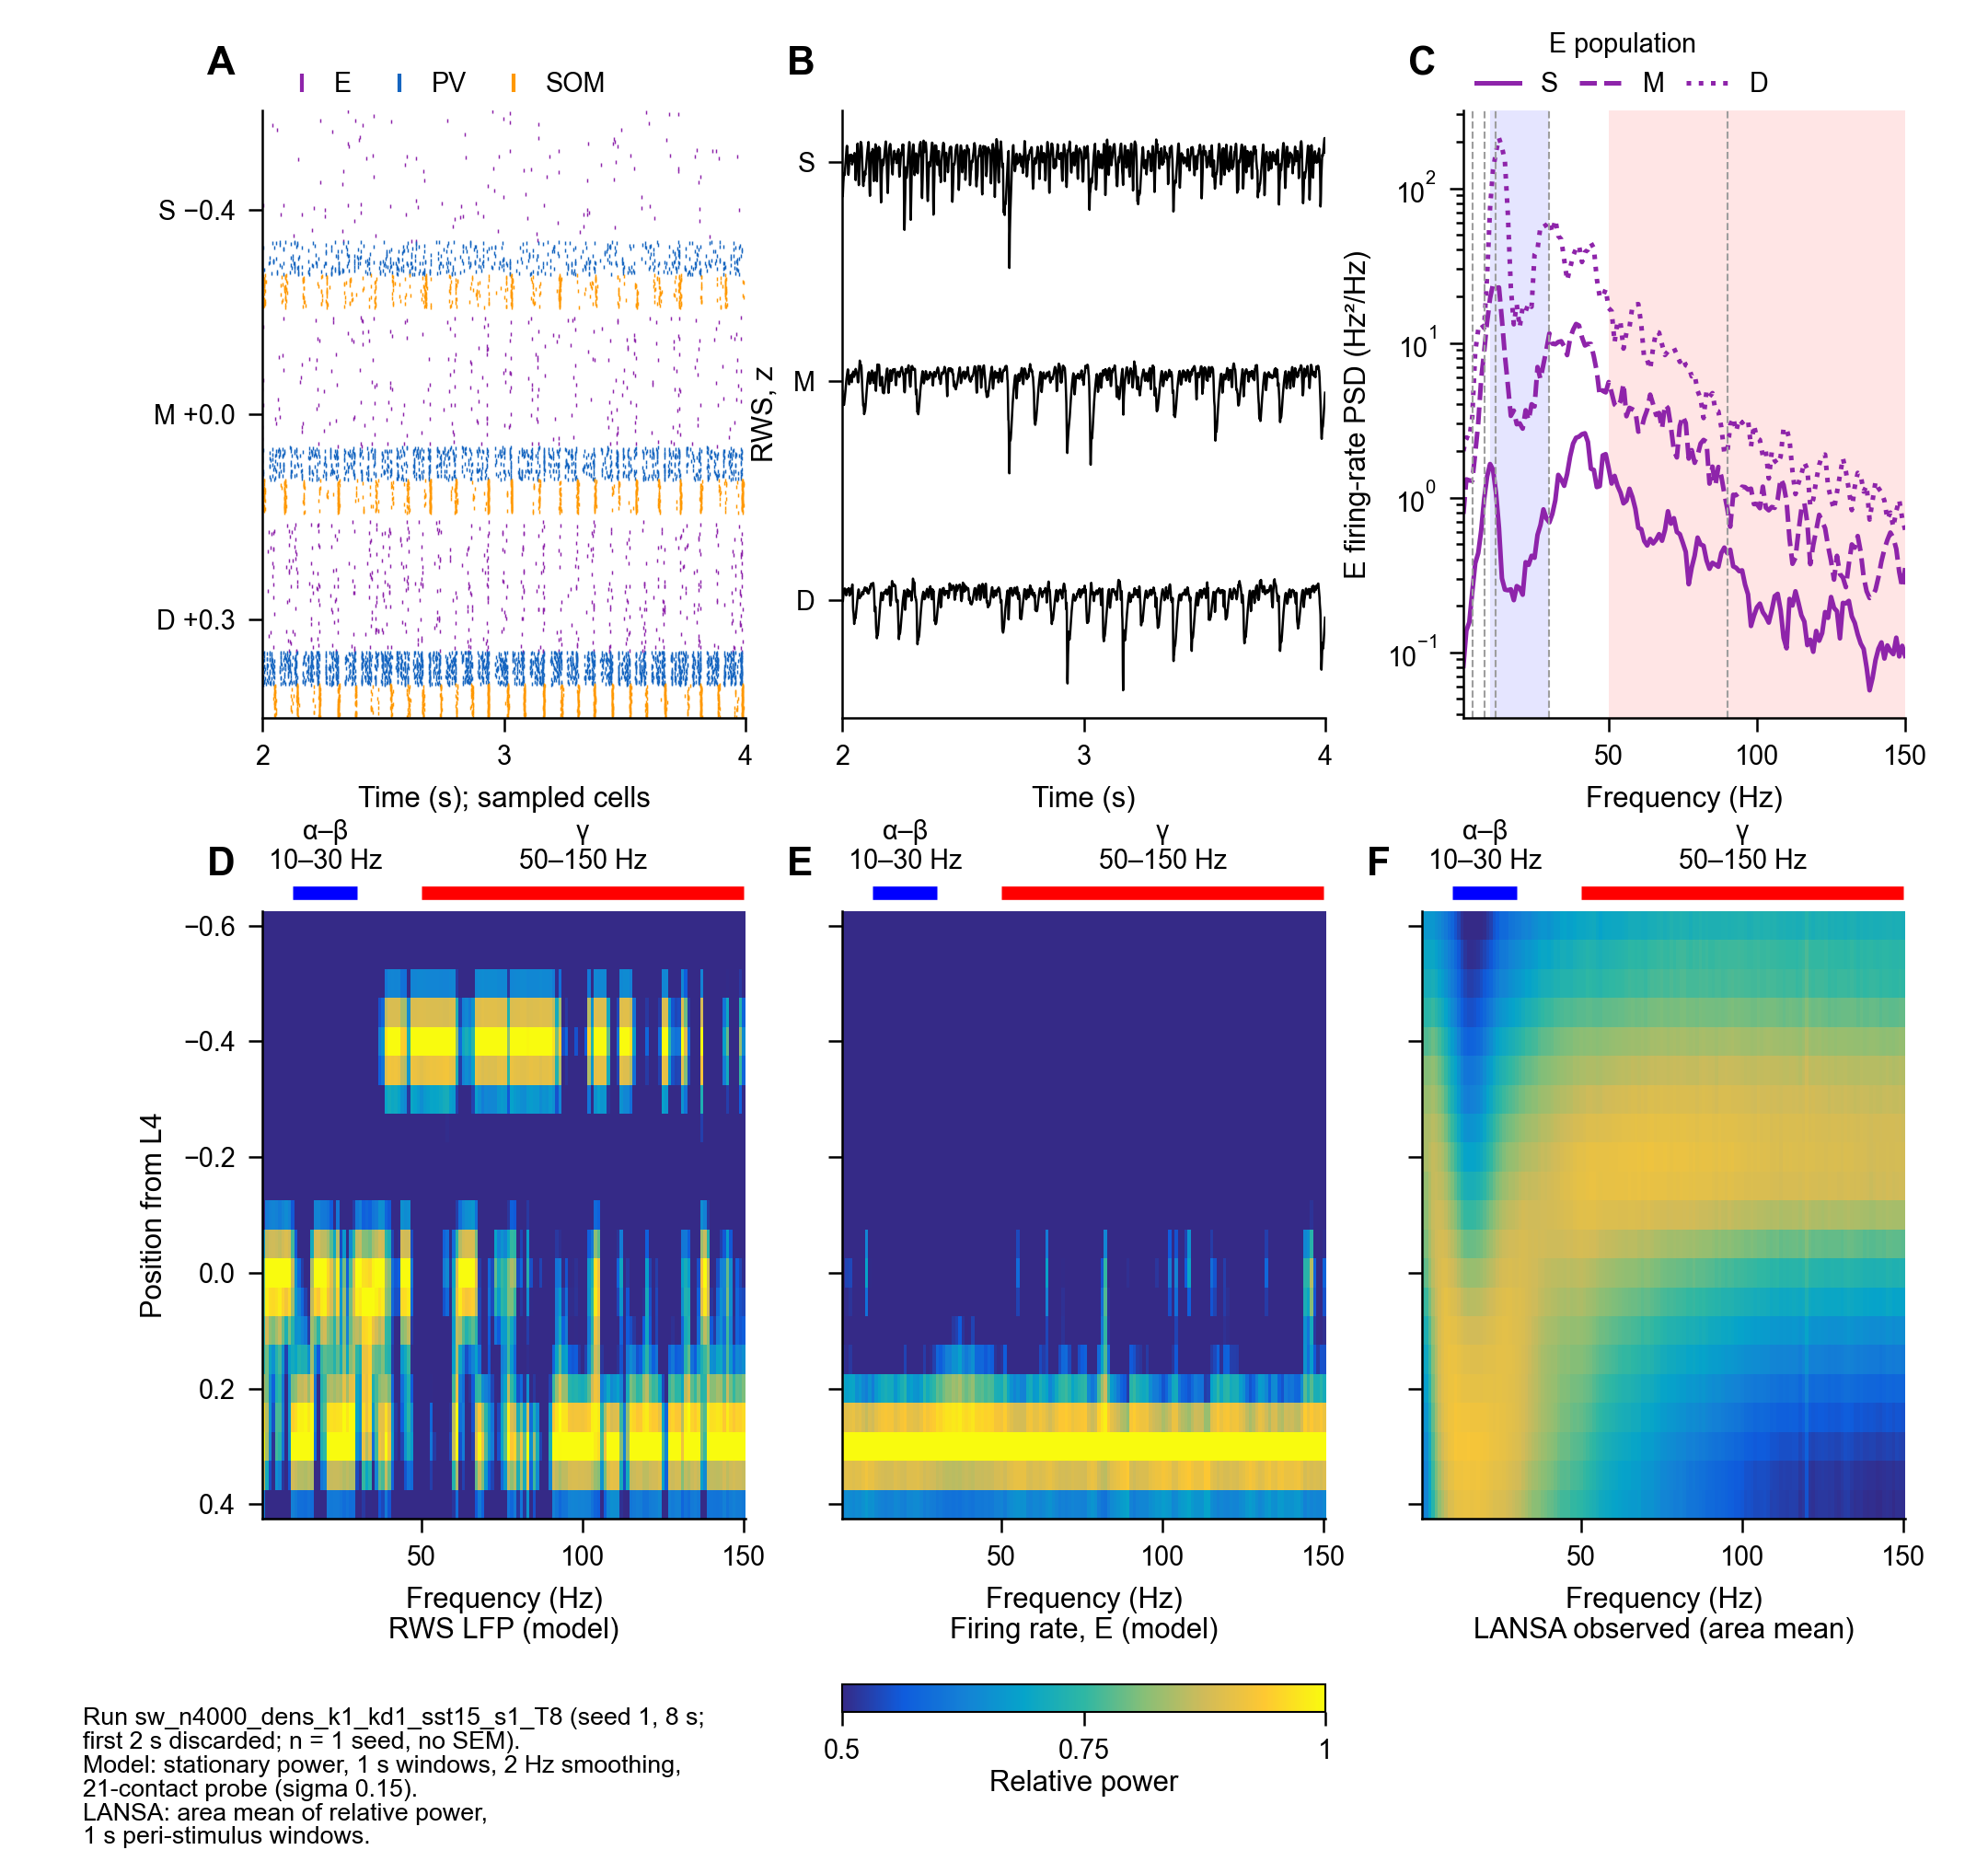
\includegraphics[width=\linewidth]{../../results/viz/paper_w3/sw_n4000_dens_k1_kd1_sst15_s1_T8_block.png}}{\pendingbox{block figure}}
\caption{Reference model, seed 1 (block file, paper\_w3). Its panels are mapped to the plan: file A (raster) = Fig 1B;
file C (per-type spectra) = Fig 1C; files D (RWS SL map) and E (firing-rate SL map) = Fig 1D; file F (observed LANSA
area map) = Fig 1E. File B (RWS traces) is not a plan panel. The letters in the image are the file's own.}
\end{figure}

\begin{figure}[tbp]
\centering
\panel{F}{../../results/laminar_e2/sw_n4000_dens_k1_kd1_sst15_s1_T8_motif.png}{0.48\linewidth}{LFP proxy and band-depth profiles}
\hfill
\panel{F (CSD)}{../../results/viz/paper_w4/sw_n4000_dens_k1_kd1_sst15_s1_T8_csd.png}{0.48\linewidth}{current-based CSD}
\caption{Reference model, seed 1. F: LFP proxy traces and band-depth profiles from the motif file (its panels d--i).
Current-based CSD from paper\_w4; CSD placements are ASSUMED (Methods). Panel letters in the image files are their own.}
\end{figure}

\subsection{Fig 2: robustness}

\todo{Fig 2 text: drive-rate sweep and seed robustness as difference maps with SSIM and Pearson r; the hierarchy panel is deferred (T7, plan section 5).}

\begin{figure}[tbp]
\centering
\stub{A: drive-rate sweep difference maps (SSIM, r)}{drive-rate sweep difference maps (SSIM, Pearson r); no difference maps written yet}
\hfill
\panel{B}{../../results/viz/paper_w6/seed_diff.png}{0.48\linewidth}{seed difference maps}\\[0.8em]
\stub{C: LANSA hierarchy (T7)}{T7 LANSA hierarchy, deferred (plan section 5, OPEN-38)}
\caption{Robustness. A: drive-rate sweep, not written. B: seed difference maps $R_a - R_b$ of the relative-power map
for each pair of seeds 1--3 at $N$ = 1000, 2000, 4000 (ladder runs), with SSIM and Pearson $r$ over all pixels
(\texttt{paper\_w6/seed\_diff.png}). Seed pairs agree (SSIM 0.62--0.71, $r$ 0.87--0.93); each seed against the
observed map gives SSIM 0.04--0.12 and $r$ 0.20--0.43. Panel C is deferred.}
\end{figure}

\subsection{Fig 3: interneuron manipulations}

\todo{Fig 3 text: PV and SST silencing, whole population and per unit; PV/SST ratio scale; VIP is stage 2.}

\begin{figure}[tbp]
\centering
\stub{A: PV silencing, whole population}{T4 PV silencing, whole population (not run)}
\hfill
\stub{B: SST silencing, whole population}{T4 SST silencing, whole population (not run)}\\[0.8em]
\stub{C: silencing per unit}{T4 per-unit silencing (not run)}
\hfill
\stub{D: PV/SST ratio scale}{T3 PV/SST ratio scale (not run)}\\[0.8em]
\stub{E: VIP}{T5 VIP, stage 2 (deferred, OPEN-36)}
\caption{Interneuron manipulations. All panels are pending; the T4 and T3 seals are in \texttt{docs/laminar\_motif/}.}
\end{figure}

\subsection{Fig 4: laminar source}

\todo{Fig 4 text: unit silencing, isolated units, graded PV silencing inside the isolated gamma unit.}

\begin{figure}[tbp]
\centering
\stub{A: unit silencing}{T4 unit silencing (not run)}
\hfill
\stub{B: isolated units}{isolated-unit runs (not run)}\\[0.8em]
\stub{C: graded PV silencing, isolated gamma unit}{graded fractions 10/25/50/75/100\% (deferred; sub-population label not built)}
\caption{Laminar source. All panels are pending.}
\end{figure}

\subsection{Fig 5: determinants}

\todo{Fig 5 text: S$\leftrightarrow$D swaps of $\rho$, in-degree, N and SST$\to$E $\tau$ on isolated units; E/I $g$ in $\{0.5, 2\}$.}

\begin{figure}[tbp]
\centering
\stub{A: S$\leftrightarrow$D swap, $\rho$}{swap of rho on isolated units (not run)}
\hfill
\stub{B: S$\leftrightarrow$D swap, in-degree}{swap of in-degree (not run)}\\[0.8em]
\stub{C: S$\leftrightarrow$D swap, N}{swap of N (not run)}
\hfill
\stub{D: SST$\to$E $\tau$}{swap of SST$\to$E $\tau$ (not run)}\\[0.8em]
\stub{E: E/I $g$}{T2 E/I, $g$ in $\{0.5, 2\}$ (not run)}
\caption{Determinants. All panels are pending.}
\end{figure}

\subsection{Fig 6: probe geometry}

\todo{Fig 6 text: tilted and offset probe readouts, scored by contrast M and by $r_\text{proto}$ minus the identical-unit control (T6; readout only, no simulation).}

\begin{figure}[tbp]
\centering
\panel{A}{../../results/viz/paper_w5/sw_n4000_dens_k1_kd1_sst15_s1_T8_probe_geometry.png}{0.48\linewidth}{probe geometry}
\hfill
\panel{B}{../../results/viz/paper_w5/lfs_n1000_s1_T8_probe_geometry.png}{0.48\linewidth}{probe geometry, n1000}\\[0.8em]
\panel{C}{../../results/viz/paper_w5/probe_summary.png}{0.96\linewidth}{T6 score summary by $\theta$ and offset}
\caption{Probe geometry, post hoc readout on saved runs. A: reference model; B: n1000 seed 1 (W5 readout outputs).
C: contrast $M_\text{arc}$ and $r_\text{proto} - r_\text{ctrl}$ by tilt and lateral offset, seed mean $\pm$ SD over
seeds 1--3 at each $N$ (\texttt{probe\_summary.png}). At offsets 0 and 0.25 the rise of $r_\text{proto} - r_\text{ctrl}$
with tilt comes from the identical-unit control falling, not from $r_\text{proto}$, which falls at $\theta = 30^\circ$.}
\end{figure}
